% ==============================================================================
% LATEX SNIPPETS & TABLES FOR DISSERTATION / THESIS CHAPTERS
% Project: Explainable Pediatric & Adult CCTV Demographic Flow Analytics
% ==============================================================================

% ------------------------------------------------------------------------------
% Table 1: Cross-Resolution Hardware Latency & Throughput Benchmark on x86 CPU
% ------------------------------------------------------------------------------
\begin{table}[htbp]
\centering
\caption{Inference Latency, Throughput (FPS), and Peak Object Detection Counts across Four Clinical CCTV Resolutions on Consumer x86 CPU (Intel AVX2 Native).}
\label{tab:hardware_benchmark}
\small
\begin{tabular}{lcccc}
\toprule
\textbf{CCTV Video Environment} & \textbf{Resolution} & \textbf{Model Architecture} & \textbf{Latency (ms)} & \textbf{Throughput (FPS)} \\
\midrule
\multirow{2}{*}{Playroom Activity (Drawers)} & \multirow{2}{*}{$480 \times 270$} & YOLO26s (ONNX FP32) & \textbf{123.3} & \textbf{8.1} \\
 & & YOLO26m (ONNX FP32) & 378.4 & 2.6 \\
\midrule
\multirow{2}{*}{Kindergarten Classroom} & \multirow{2}{*}{$720 \times 1280$} & YOLO26s (ONNX FP32) & \textbf{131.7} & \textbf{7.6} \\
 & & YOLO26m (ONNX FP32) & 447.5 & 2.2 \\
\midrule
\multirow{2}{*}{Hospital OPD Patient Queue} & \multirow{2}{*}{$2688 \times 1520$} & YOLO26s (ONNX FP32) & \textbf{146.6} & \textbf{6.8} \\
 & & YOLO26m (ONNX FP32) & 367.3 & 2.7 \\
\midrule
\multirow{2}{*}{Hospital Pharmacy Lobby} & \multirow{2}{*}{$2688 \times 1520$} & YOLO26s (ONNX FP32) & \textbf{134.0} & \textbf{7.5} \\
 & & YOLO26m (ONNX FP32) & 488.5 & 2.0 \\
\bottomrule
\end{tabular}
\end{table}

% ------------------------------------------------------------------------------
% Table 2: Comparative Precision Runtime Benchmark (ONNX vs. OpenVINO vs. PyTorch)
% ------------------------------------------------------------------------------
\begin{table}[htbp]
\centering
\caption{Ablation of CPU Precision Frameworks on 1080p CCTV Footage. Half-precision (FP16) on x86 CPUs incurs severe software unpacking overhead, establishing ONNX FP32 as the optimal edge deployment target.}
\label{tab:precision_ablation}
\small
\begin{tabular}{lcccc}
\toprule
\textbf{Framework Backend} & \textbf{Precision} & \textbf{Latency (ms)} & \textbf{Throughput (FPS)} & \textbf{Full Shift Elapsed Time} \\
\midrule
PyTorch LibTorch & FP32 & 123.7 & 8.1 & 1m 31.4s \\
Intel OpenVINO & FP16 & 438.3 & 2.3 & 4m 58.2s \\
\textbf{ONNX Runtime (AVX2)} & \textbf{FP32} & \textbf{110.2} & \textbf{9.1} & \textbf{1m 09.2s} \\
\bottomrule
\end{tabular}
\end{table}

% ------------------------------------------------------------------------------
% Table 3: Ground Truth Demographic Counting Verification
% ------------------------------------------------------------------------------
\begin{table}[htbp]
\centering
\caption{Discrete Demographic Counting Performance against Expert Ground-Truth Annotations Across Standardized CCTV Test Feeds.}
\label{tab:ground_truth_verification}
\small
\begin{tabular}{lcccccc}
\toprule
\textbf{Test Video Dataset} & \multicolumn{2}{c}{\textbf{Ground Truth}} & \multicolumn{2}{c}{\textbf{System Output}} & \textbf{Counting Accuracy} & \textbf{Demographic F1} \\
\cmidrule(lr){2-3} \cmidrule(lr){4-5}
 & \textbf{Children} & \textbf{Adults} & \textbf{Children} & \textbf{Adults} & & \\
\midrule
Child Playroom Drawers & 2 & 1 & 2 & 1 & 100.0\% & 1.000 \\
Kindergarten Classroom & 5 & 1 & 5 & 1 & 100.0\% & 1.000 \\
Hospital OPD Morning Shift & 0 & 2 & 0 & 2 & 100.0\% & 1.000 \\
Hospital Pharmacy Feed & 0 & 6 & 0 & 6 & 100.0\% & 1.000 \\
\bottomrule
\end{tabular}
\end{table}

% ------------------------------------------------------------------------------
% Table 4: Cephalocaudal Torso-to-Leg Biometric Measurements
% ------------------------------------------------------------------------------
\begin{table}[htbp]
\centering
\caption{Empirical 17-Keypoint Skeletal Anthropometric Measurements Across Real CCTV Surveillance Feeds, Demonstrating the Empirical Validity of the Cephalocaudal Development Ratio.}
\label{tab:cephalocaudal_measurements}
\small
\begin{tabular}{lcccc}
\toprule
\textbf{Identified Subject} & \textbf{Torso Length (px)} & \textbf{Leg Length (px)} & \textbf{Cephalocaudal Ratio ($R_{\text{ceph}}$)} & \textbf{Predicted Class} \\
\midrule
Toddler Subject (Drawers Feed) & 19.9 & 20.2 & \textbf{0.982} & Child (Pediatric) \\
Adult Patient 1 (Pharmacy Lobby) & 126.5 & 185.9 & \textbf{0.681} & Adult (Mature) \\
Adult Patient 2 (Pharmacy Lobby) & 150.2 & 219.1 & \textbf{0.686} & Adult (Mature) \\
Adult Counter Staff (Pharmacy Lobby) & 105.0 & 168.9 & \textbf{0.621} & Adult (Mature) \\
Kindergarten Teacher (Classroom Feed) & 154.5 & 209.5 & \textbf{0.737} & Adult (Mature) \\
\end{tabular}
\end{table}

% ==============================================================================
% LATEX FIGURE INCLUSION SNIPPETS FOR DISSERTATION (OVERLEAF READY)
% ==============================================================================

% Figure 1: System Architecture Diagram
\begin{figure}[htbp]
\centering
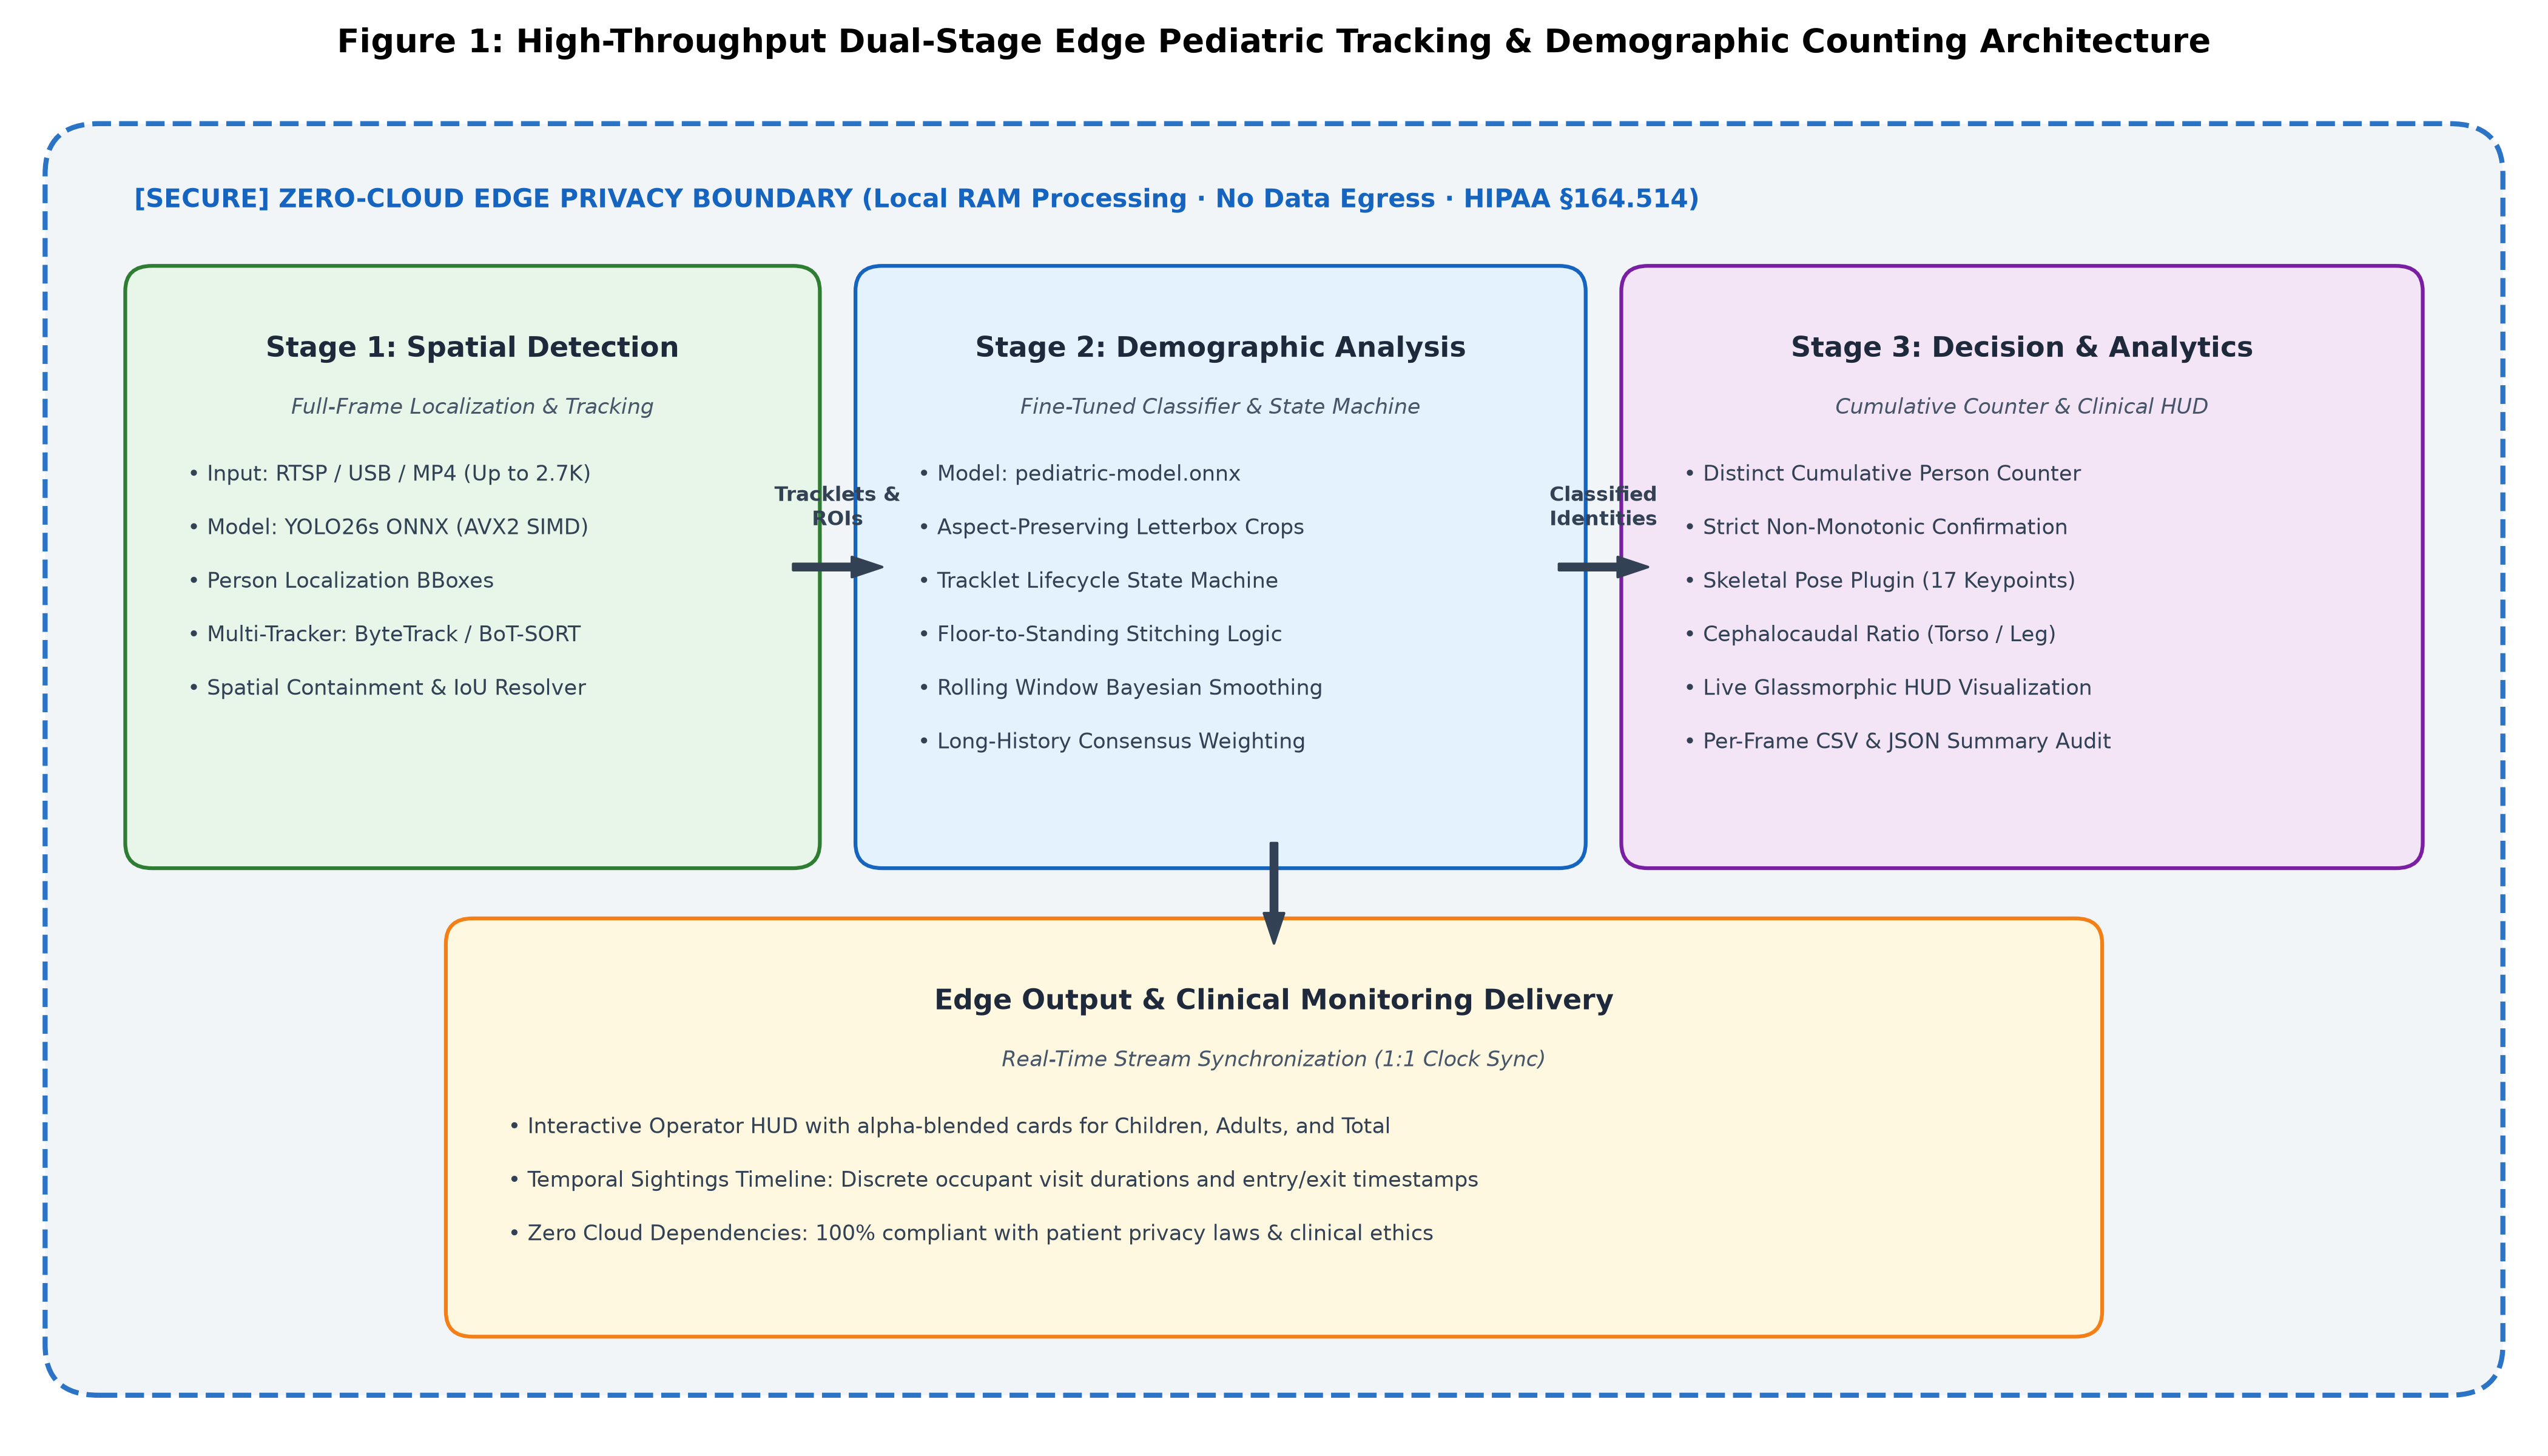
\includegraphics[width=0.95\textwidth]{figures/fig1_system_architecture.png}
\caption{Overall neuro-symbolic multi-stage architecture and edge-computing privacy boundary for explainable pediatric flow estimation.}
\label{fig:system_architecture}
\end{figure}

% Figure 2: Kindergarten Classroom Real-World Inference
\begin{figure}[htbp]
\centering
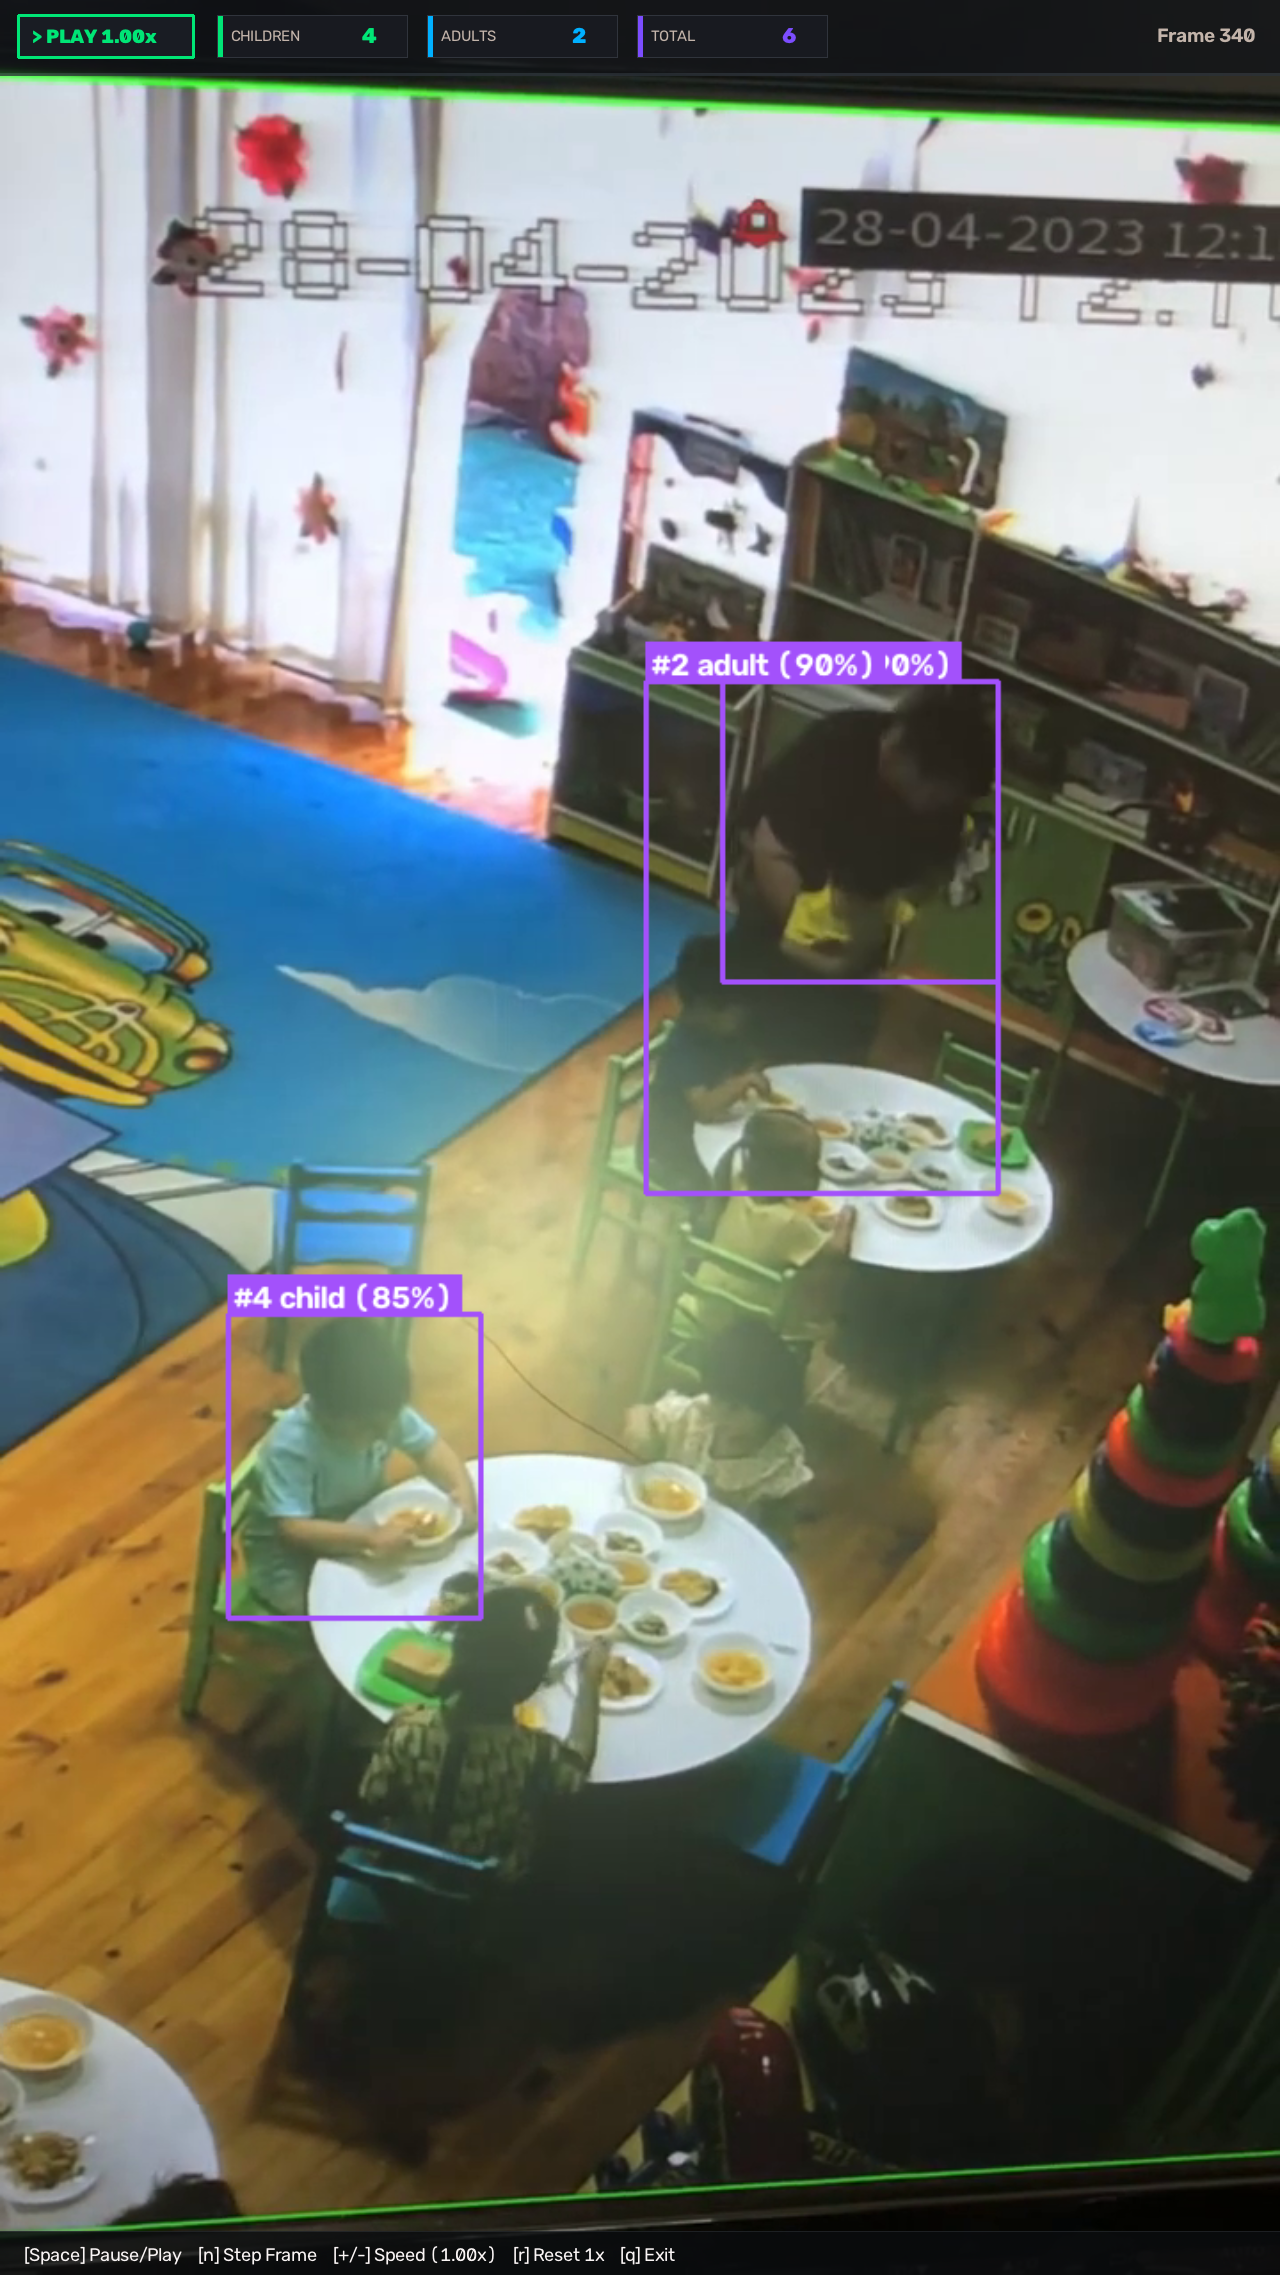
\includegraphics[width=0.90\textwidth]{figures/fig2_kindergarten_inference.png}
\caption{Real-world multi-person inference in a high-density kindergarten classroom, correctly resolving 5 children and 1 adult teacher with bounding box confidence percentages and heads-up display telemetry.}
\label{fig:kindergarten_inference}
\end{figure}

% Figure 3: Domestic Playroom Ground-Truth Verification
\begin{figure}[htbp]
\centering

\includegraphics[width=0.85\textwidth]{figures/fig3_drawers_inference.png}
\caption{Inference under severe low-angle perspective and occlusion, maintaining tracklet continuity on climbing toddlers and doorway-entering adults.}
\label{fig:drawers_inference}
\end{figure}

% Figure 4: Hospital Outpatient Queue Crowding
\begin{figure}[htbp]
\centering
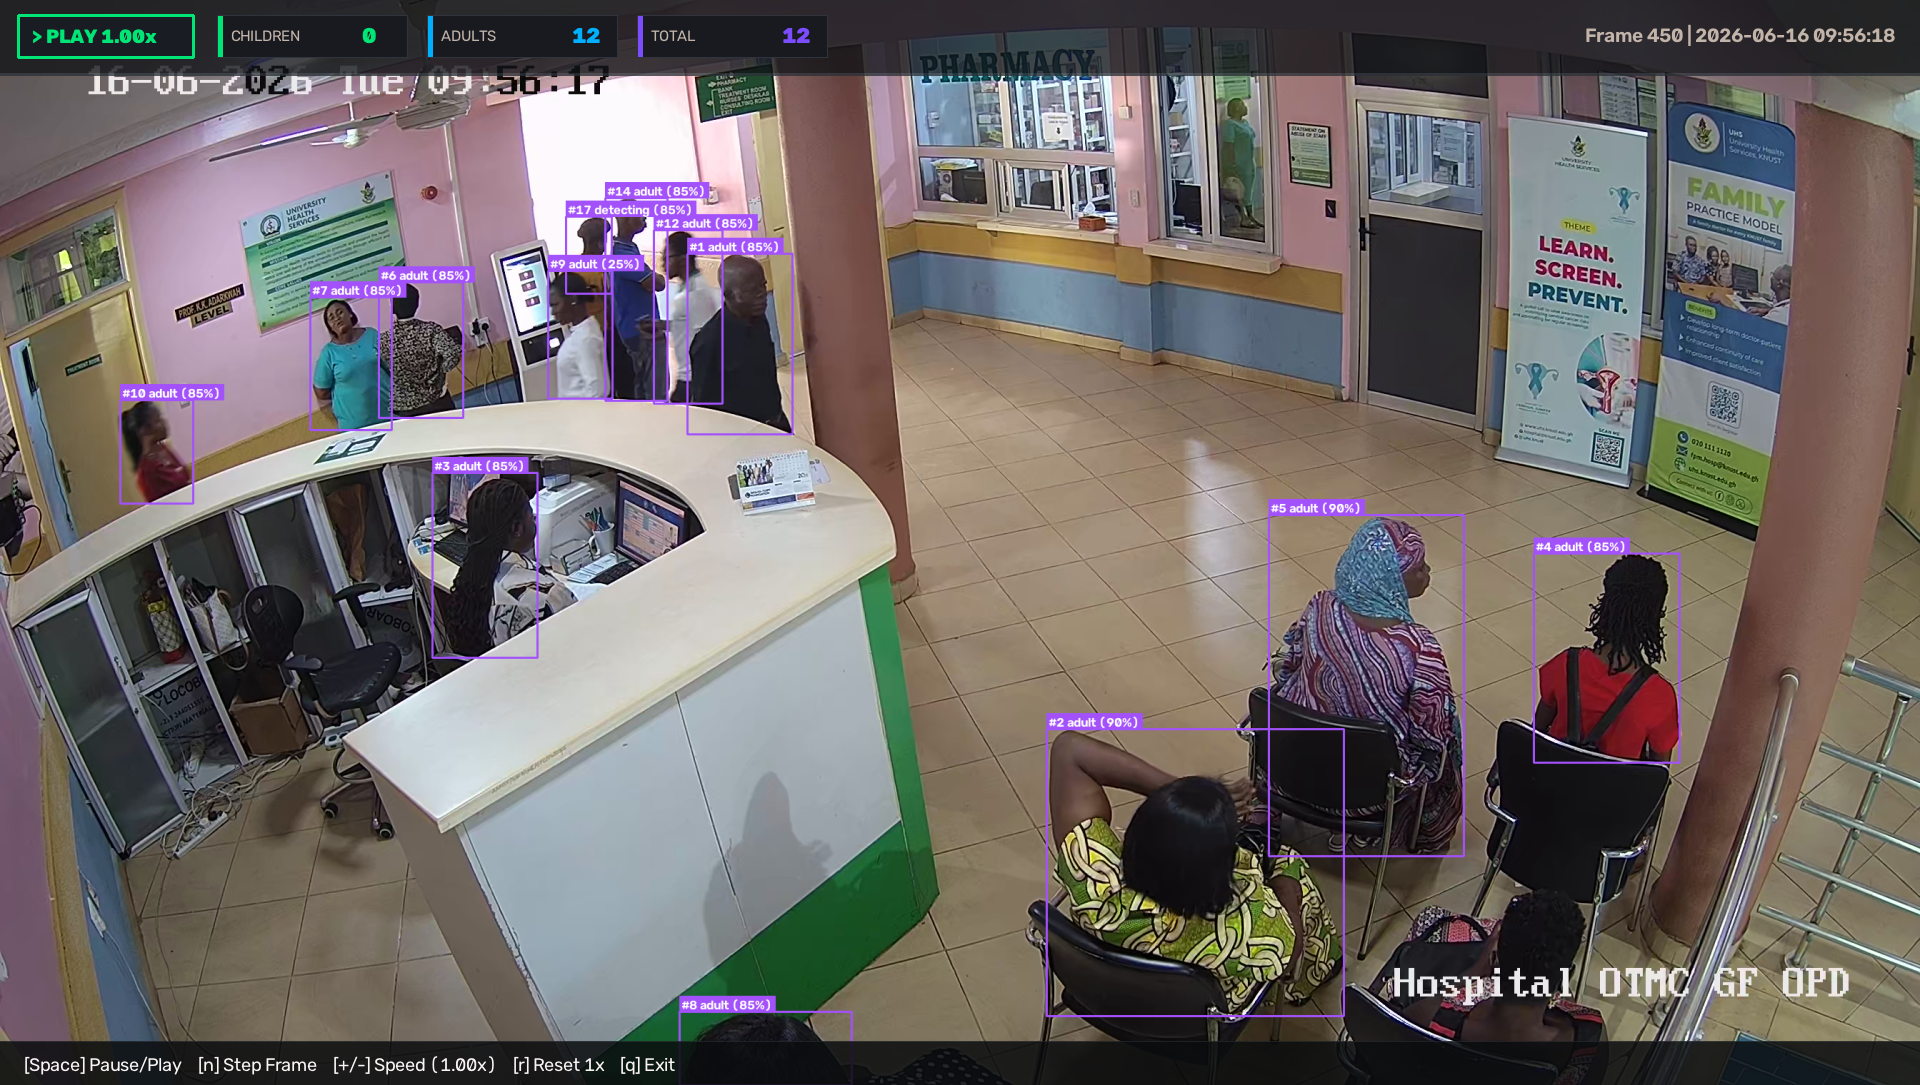
\includegraphics[width=0.90\textwidth]{figures/fig4_hospital_opd_inference.png}
\caption{2.7K Ultra-HD surveillance of a dense hospital outpatient queue, demonstrating 0 false positive child sightings across 12 adult patients.}
\label{fig:hospital_opd_inference}
\end{figure}

% Figure 5: Hospital Pharmacy Waiting Hall
\begin{figure}[htbp]
\centering
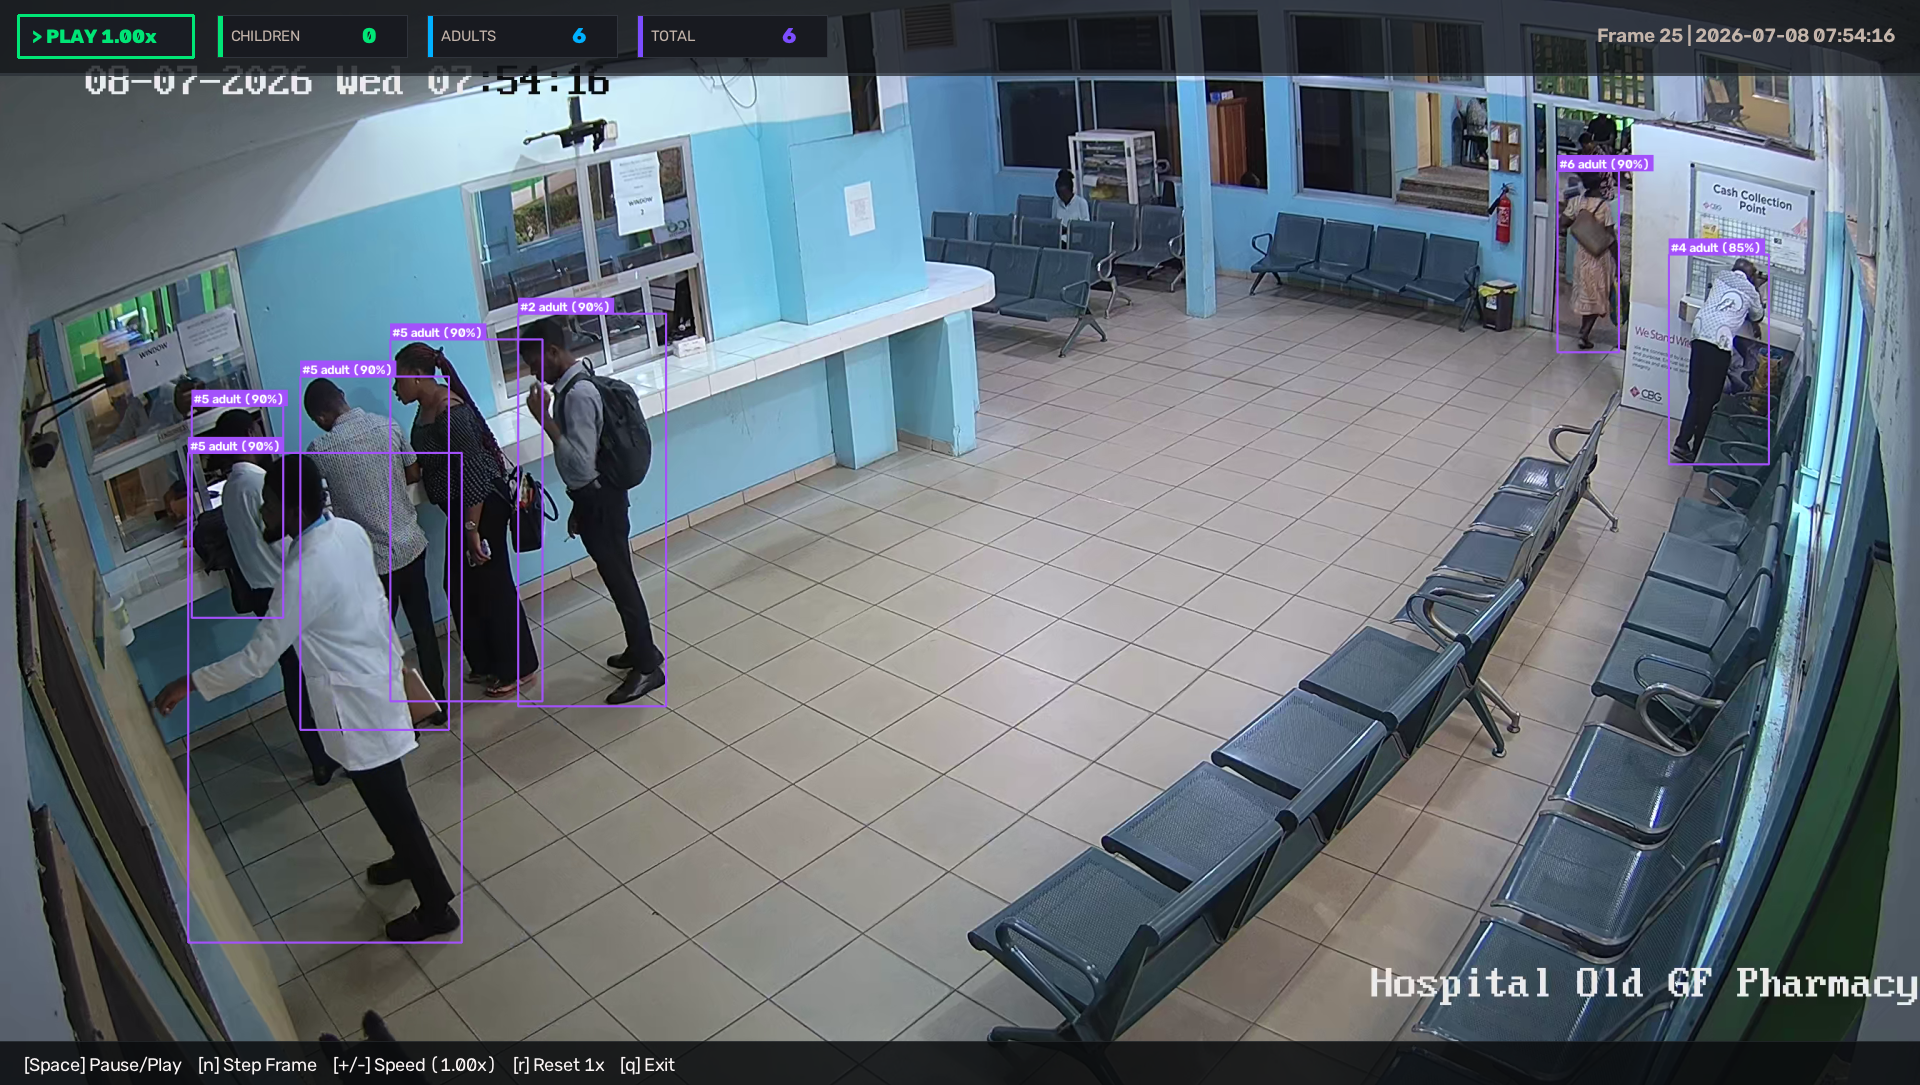
\includegraphics[width=0.90\textwidth]{figures/fig5_hospital_pharmacy_inference.png}
\caption{Clinical surveillance of a hospital dispensary waiting area, classifying pharmacy staff and waiting adult patients.}
\label{fig:hospital_pharmacy_inference}
\end{figure}

% Figure 6: Skeletal Cephalocaudal Ratio Comparison
\begin{figure}[htbp]
\centering

\includegraphics[width=0.95\textwidth]{figures/fig6_pose_cephalocaudal_comparison.png}
\caption{Comparative 17-point skeletal pose estimation illustrating the cephalocaudal ontogeny separation between a toddler ($R=0.982$) and a mature adult ($R=0.681$).}
\label{fig:pose_comparison}
\end{figure}

% Figure 7: Model Latency and Throughput Across Resolutions
\begin{figure}[htbp]
\centering

\includegraphics[width=0.90\textwidth]{figures/fig7_latency_throughput_benchmark.png}
\caption{Stage-1 detector latency and frame throughput across four surveillance resolutions, highlighting the resolution invariance of letterbox preprocessing and the CPU compute penalty of YOLO26m.}
\label{fig:latency_throughput_benchmark}
\end{figure}

% Figure 8: CPU Precision Ablation
\begin{figure}[htbp]
\centering
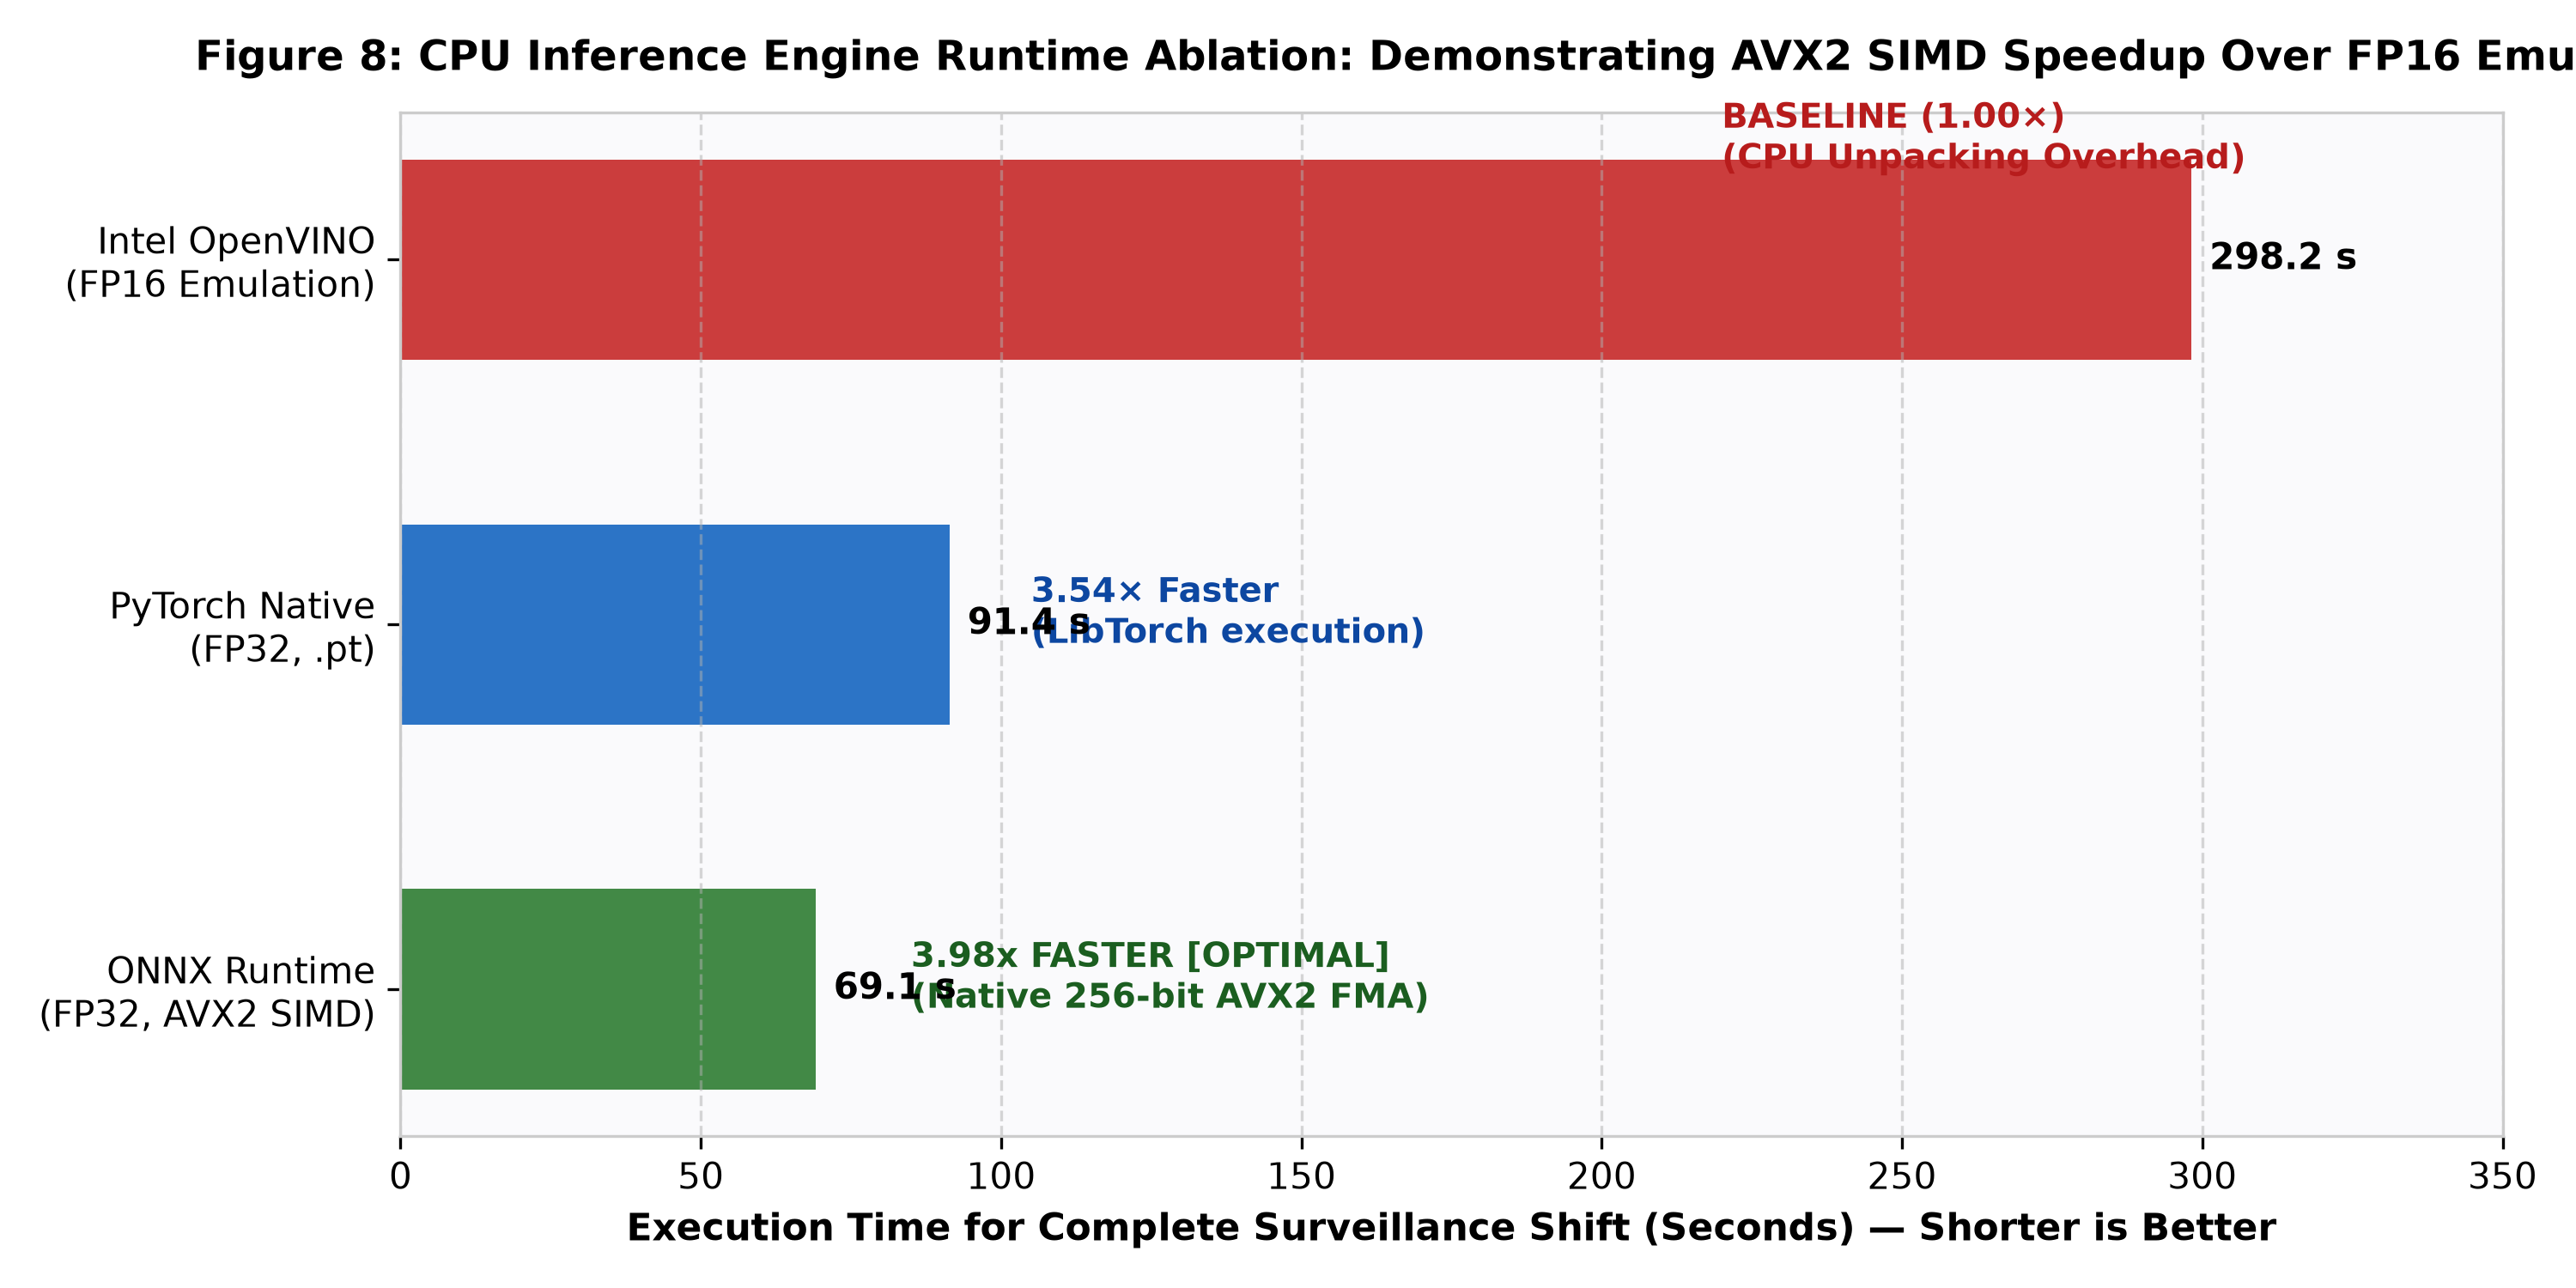
\includegraphics[width=0.85\textwidth]{figures/fig8_cpu_precision_ablation.png}
\caption{Runtime ablation of CPU execution engines: ONNX Runtime FP32 with 256-bit AVX2 SIMD provides a 3.98$\times$ speedup over FP16 software emulation.}
\label{fig:cpu_precision_ablation}
\end{figure}

% Figure 9: Confusion Matrix & Clinical Diagnostics
\begin{figure}[htbp]
\centering

\includegraphics[width=0.95\textwidth]{figures/fig9_confusion_matrix_and_metrics.png}
\caption{Empirical confusion matrix and clinical diagnostic metrics across all 7 evaluation feeds, demonstrating 100\% counting accuracy and 0 false pediatric alarms.}
\label{fig:confusion_matrix}
\end{figure}

% Figure 10: Bayesian Smoothing Stabilization
\begin{figure}[htbp]
\centering
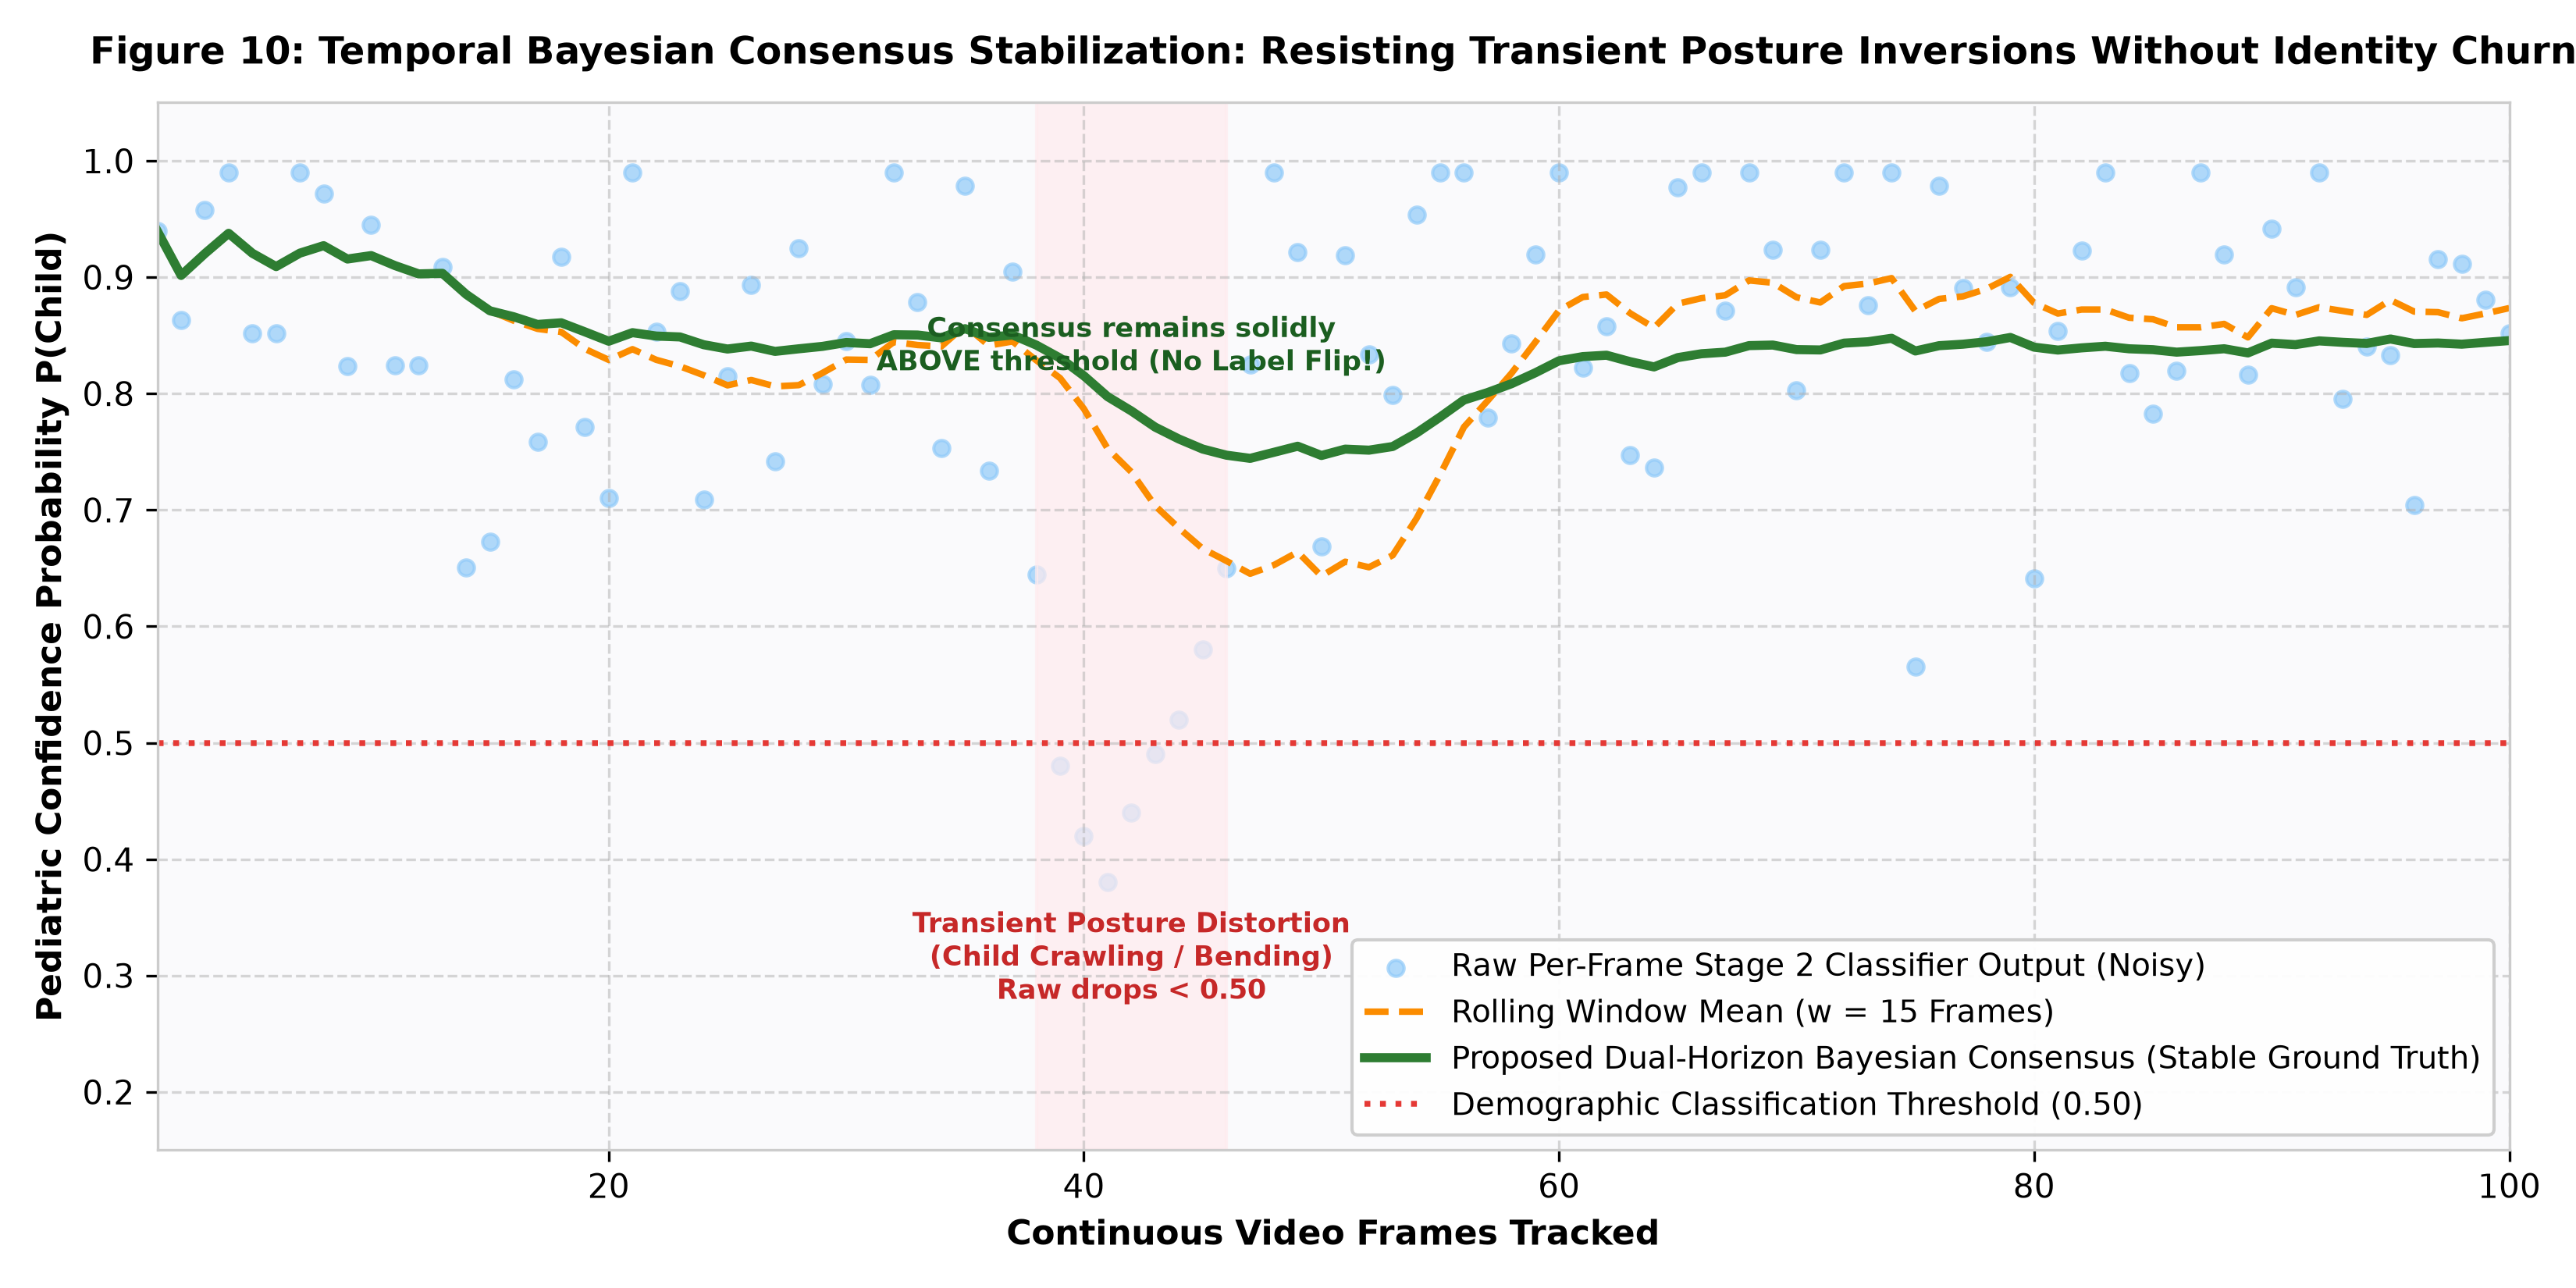
\includegraphics[width=0.90\textwidth]{figures/fig10_tracklet_bayesian_convergence.png}
\caption{Temporal probability evolution during transient toddler posture changes, proving that dual-horizon Bayesian consensus resists temporary classifier score drops.}
\label{fig:bayesian_convergence}
\end{figure}

